% !TeX spellcheck = en_GB
% ***************************************************** %
\section{Mini-batch gradient descent variants}\label{sc:sgds}
% ***************************************************** %

In this section we tackle the algorithmic part, specifically the SGD-type is the Mini-batch Gradient Descent where the mini-batch size $M$ is greater than 1 and much less than the dataset size, i.e. $1<\abs{B}=M\ll N$, however, we will call it SGD.

%The SGD algorithm performs steps of the following form
%\[
%w^{k+1}=w^k+\alpha_kd_k,\quad d_k=-\nabla f_{i_k}(w^k)
%\]
%where the direction $d_k$ is equal to the \emph{anti-gradient} evaluated on the considered samples (a random mini-batch extracted from the dataset), knowing that $\numberset{E}\bigl[\nabla f_{i_k}(w^k)\bigr]=\nabla\func(w)$, $d_k$ is a \emph{descent direction} on average, so the objective function doesn't decrease necessarily at each step. Also, for the global convergence, the algorithm can start from an arbitrary $w^0\in\R^{(p+1)}$.

%Using this step-size form, without a line search method for choosing the optimal step-size $\alpha_k$, the objective function value doesn't decrease necessarily at each step, thus making the method \emph{non-monotonous}.

In order to use the algorithm, it is necessary to make further assumptions on the objective function and the gradients (how far the gradient samples are from the \emph{true gradients})
\begin{itemize}
%\item the function $f$ in problem~\eqref{eq:opt-prob} has a \emph{finite-sum structure}, that is the common machine learning setting;
\item the objective function in problem~\ref{eq:opt-prob} is a loss function plus a quadratic regularization term, $f$ is bounded below by some value $f^\ast$ as we can also see in figure~\ref{subfig:log-loss};
\item for some constant $G>0$ the magnitude of all gradients samples is bounded $\forall w\in\R^{(p+1)}$, by $\norma{\nabla f_i(w)}\leq G$;
\item other than twice continuously differentiable, we assume that $f$ has Lipschitz-continuous gradients with constant $L>0$, one can also say that $f$ is $L\text{-smooth}$.
\end{itemize}

The algorithm is globally convergent, so the starting point will be an arbitrary $w^0\in\R^{(p+1)}$.

\subsubsection*{Stopping criterion and failures}

Regarding the implementation of the algorithm, it is essential to define a stopping criterion. Given a small $\epsilon>0$ the chosen criterion is as follows
%\begin{subequations}
%\begin{align}
%\norma{\nabla\func(w^k)} &\leq \epsilon \label{eq:stopping1} \\
%\norma{\nabla\func(w^k)} &\leq \epsilon\bigl(1+\abs{\underbrace{\func(w^k)}_{\geq0\,\forall w^k}}\bigr)=\epsilon\bigl(1+\func(w^k)\bigr) \label{eq:stopping2}
%\end{align}
%\end{subequations}
%\[
%\norma{\nabla\func(w^k)}\leq
%\begin{cases}
%\epsilon \\
%\epsilon\bigl(1+\abs{\func(w^k)}\bigr)=\epsilon\bigl(1+\func(w^k)\bigr)
%\end{cases}
%\]
\begin{equation}\label{eq:stopping}
\norma{\nabla\func(w^k)}\leq\epsilon
\end{equation}
unlike the first one, the second is independent from the scale of the objective function. Note that the criterion uses the full gradient.

Other than the stopping criterion, we can add conditions of premature termination like
\begin{itemize}
\item exceeding a threshold for the epochs number $k^\ast$ or function and gradient evaluations;
\item internal failures when computing $w^{k+1}$, for example exceeding $q^\ast$ iterations during the line search (as you will se later, for the step-size $\alpha$ as well as the momentum term $\beta$).
\end{itemize}


\subsubsection*{Mini-batch gradient}

Now we spend few words about the notation and the computation of the mini-batch gradient. Being on epoch $k$ at iteration $t$, a model update starting from a $w^k$ has the following form
\begin{equation}\label{eq:sgd-step}
y_{t+1}=y_t+\alpha_td_t
\end{equation}
the update uses information from the mini-batch $B_t$ in the direction $d_t$ and the step-size $\alpha_t$ follows a certain rule.\footnote{\emph{Iterations} is defined as the total number of mini-batches extracted from the dataset, while one \emph{epoch} is when the entire dataset is passed forward. The counter for the mini-batch currently processed is $t$ while $k$ is for the epoch.}

%The direction is an expression involving the gradient, so we want to compute the gradient w.r.t. $y_t$ on the mini-batch $B_t$ whose indices are randomly chosen $i_t\subset\set{1,\dots,N}$
%\begin{equation*}
%%\begin{split}
%%\nabla f_{i_t}(y_t) &= \frac{1}{M}\sum_{j\in B_t}\nabla f_j(y_t)\\
%% &= \frac{1}{M}\sum_{j\in B_t}\bigl(x^{(j)}r_j+\lambda y\bigr) \\
%% &= \frac{1}{M}\biggl(\sum_{j\in B_t}x^{(j)}r_j+M\lambda y\biggr) \\
%% &= \frac{1}{M}\bigl(\underbrace{Xr}_{i_t\in B_t}+\lambda' y\bigr)
%%\end{split}
%\begin{split}
%\nabla f_{i_t}(y_t) &= \frac{1}{M}\sum_{i\in B_t}\nabla f_i(y_t)=\frac{1}{M}\sum_{i\in B_t}\bigl(x^{(i)}r_i+\lambda y\bigr)= \frac{1}{M}\biggl(\sum_{i\in B_t}x^{(i)}r_i+M\lambda y\biggr) \\
%&= \frac{1}{M}\bigl(\underbrace{Xr}_{i\in B_t}+\lambda'y\bigr)
%\end{split}
%\end{equation*}
%the expression is the same as the full gradient~\eqref{subeq:jacobian} except that the dataset matrix contains just the mini-batch samples (and so the $r$ vector), and the regularization coefficient is redefined as $\lambda'=M\lambda$ where $M$ is the size of the considered mini-batch. This expression will be used in the implementation.

The direction is an expression involving the gradient, so we want to compute the gradient w.r.t. $y_t$ on the mini-batch $B_t$ whose indices are randomly chosen $i_t\subset\set{1,\dots,N}$. Knowing that $\nabla f_i(w^k)=x^{(i)}r_i+\lambda w^k$
\begin{equation}\label{eq:mini-grad}
\begin{split}
\nabla f_{i_t}(y_t) &= \frac{1}{M}\sum_{i\in B_t}\nabla \ell_i(y_t)+\lambda\nabla\Omega(y_t) \\
 &= \frac{1}{M}\underbrace{Xr}_{i\in B_t}+\lambda y_t
\end{split}
\end{equation}
the expression is the same as the full gradient~\eqref{subeq:jacobian} except that the dataset matrix contains just the mini-batch samples, so the $r$ vector.

%Being on epoch $k$ and iteration $t$, the next ``internal'' weight obtained from the mini-batch $B_t$, whose indices are $i_t$, is

%where $\alpha_t$ is the step-size according to a specific schedule. So the mini-batch gradient

%Nothing changes when the algorithm is SGDM
%\begin{equation}\label{eq:sgdm-step}
%y_{t+1}=y_t+\alpha_td_t,\quad d_t=-\bigl((1-\beta)\nabla f_{i_t}(y_t)+\beta d_{t-1}\bigr)
%\end{equation}

% ---------------------------------------------------- %
\subsection{Stochastic gradient descent}\label{subsc:sgd}
% ---------------------------------------------------- %

The basic SGD version has the following update rule
\begin{equation}\label{eq:sgd-base}
y_{t+1}=y_t-\alpha_t\nabla f_{i_t}(y_t)
\end{equation}
so the direction is defined as $d_t=-\nabla f_{i_t}(y_t)$ that is the \emph{anti-gradient} evaluated on the considered mini-batch, we know that on average is a \emph{descent direction} so the objective function doesn't decrease necessarily at each step.

Given an initial step-size $\alpha_0\in\R^+$, the first two basic version are 
\begin{itemize}
\item \texttt{SGD-Fixed}: constant step-size $\alpha_t=\alpha_0$;
\item \texttt{SGD-Decreasing}: decreasing step-size $\alpha_t=\frac{\alpha_0}{k+1}$.
\end{itemize}
The first choice sees the same step-size between the epochs and so the iterations. The second choice changes the step-size at every epoch, while being constant between iterations, that particular form ensures the convergence. This two version are shown in algorithm~\vref{alg:SGD-F-D-M} which is a general version that includes the momentum term (see section~\ref{subsc:sgdm}), for this two cases we set $\beta_0=0$.

\subsubsection{Stochastic line search}

%Other than $\mathcal{L}_0=\set{w\in\R^{(p+1)}\mid\func(w)\leq\func(w^0)}$ being a \emph{compact set}, since the function is coercive (see\dots)
Now we move forward to the approach by~\textcite{vaswani_painless_2019}. For using the algorithm proposed by the paper, one more assumption is needed, that is, the model is able to \emph{interpolate} the data, this property requires that the gradient w.r.t. each samples converges to zero at the optimal solution
\[
\text{if}\,\,\,w^\ast\mid\nabla\func(w^\ast)=0\Rightarrow\nabla f_i(w^\ast)=0\,\,\,\forall i=1,\dots,N
\]
% a property that the log-loss satisfies

The proposed approach applies the Armijo line search to the SGD algorithm at every iteration, specializing the sufficient reduction condition in the context of finite-sum problems. Hence the \emph{Armijo condition} has the following form
\begin{equation}\label{eq:mini-armijo}
f_{i_t}\bigl(y_t-\alpha_t\nabla f_{i_t}(y_t)\bigr)\leq f_{i_t}(y_t)-\gamma\alpha_t\norma{\nabla f_{i_t}(y_t)}^2
\end{equation}
the coefficient $\gamma$ is an hyper-parameter that will be set to $1/2$ for convergence properties stated by the paper.

%Referring to the notation in~\eqref{eq:sgd_step}, the \emph{Armijo condition} has the following form
%\[
%\func(w^{k+1})\leq\func(w^k)+\gamma\alpha_k\nabla\func(w^k)^Td_k\Rightarrow
%f_{i_k}(w^{k+1})\leq f_{i_k}(w^k)+\gamma\alpha_k\nabla f_{i_k}(w^k)^Td_k
%\]
%so, when it comes to SGD we obtain
%\begin{equation}\label{eq:armijo-sls}
%f_{i_k}\bigl(w^k-\alpha_k\nabla f_{i_k}(w^k)\bigr)\leq f_{i_k}(w^k)-\gamma\alpha_k\nabla\norma{f_{i_k}(w^k)}^2
%\end{equation}
%as already said, $d_k$ is a \emph{descent direction}. The constant $\gamma$ is an hyper-parameter set to $1/2$ for convergence properties in the strongly-convex case.

As the standard Armijo method, the proposed line search uses a \emph{backtracking} technique that iteratively decreases the initial step-size $\alpha_0\in\R^+$ by a constant factor $\delta$ usually set to $1/2$ until the condition is satisfied.

The authors also gave heuristics in order to avoid unnecessary function evaluations by \emph{restarting} at each iteration the step-size, to the previous multiplied by the factor $a^{M/N}/\delta$, see algorithm~\vref{alg:reset-step}.

The SGD with Armijo Line Search \texttt{SGD-Armijo} is shown in algorithm~\vref{alg:SGD-SLS-M}.

% ---------------------------------------------------- %
\subsection{Adding momentum term}\label{subsc:sgdm}
% ---------------------------------------------------- %

The iteration performed over the mini-batches is~\eqref{eq:sgd-step} what differs from the previous versions is the direction that is
\[
d_t=-\bigl((1-\beta_0)\nabla f_{i_t}(y_t)+\beta_0d_{t-1}\bigr)
\]
in a finite-sum problem the momentum term lies in a specific range $\beta_0\in(0,1)$ and is a constant value, the algorithm that uses this direction is the \texttt{SGDM}, the resulting iteration
\begin{equation}\label{eq:sgdm-step}
y_{t+1}=y_t-\alpha_t\bigl((1-\beta)\nabla f_{i_t}(y_t)+\beta d_{t-1}\bigr)
\end{equation}
which is applied as the general update rule in algorithm~\vref{alg:SGD-F-D-M}, in this case the momentum term is constant $\beta=\beta_0$. To be clear we have the following cases
%\begin{center}
%\begin{tikzpicture}[-latex]
%\node (A) at (0,0) {$y_{t+1}=y_t-\alpha_t\bigl((1-\beta_0)\nabla f_{i_t}(y_t)+\beta_0d_{t-1}\bigr)$};
%\node[text width=3cm] (B) at ($(A.east) + (10:10em)$) {\eqref{eq:sgd-base} \texttt{SGD-Fixed},\\\texttt{SGD-Decreasing}};
%\node (C) at ($(A.east) + (-10:9em)$) {\eqref{eq:sgdm-step} \texttt{SGDM}};
%\draw (A.east) -- node[above=1ex] {$\beta_0=0$} (B.west);
%\draw (A.east) -- node[below=1ex] {$\beta_0\in(0,1)$} (C.west);
%\end{tikzpicture}
%\end{center}
\begin{center}
\begin{tikzpicture}[-latex]
\node (A) at (0,0) {$y_{t+1}=y_t-\alpha_t\bigl((1-\beta_0)\nabla f_{i_t}(y_t)+\beta_0d_{t-1}\bigr)$};
\node[text width=3cm] (B) at ($(A.east) + (10:10em)$) {\eqref{eq:sgd-base} \texttt{SGD-Fixed},\\\texttt{SGD-Decreasing}};
\node (C) at ($(A.east) + (-10:9em)$) {\eqref{eq:sgdm-step} \texttt{SGDM}};
\draw (A.east) -- ++(0.5,{10em*sin(10)}) -- node[above] {$\beta_0=0$} (B.west);
\draw (A.east) -- ++(0.5,{-9em*sin(10)}) -- node[below] {$\beta_0\in(0,1)$} (C.west);
\end{tikzpicture}
\end{center}

\subsubsection{Stochastic line search}

As the paper by~\textcite{fan_msl_2023} says, when using the momentum term together with a line search, $\beta_0$ complicates the selection of a suitable step-size. The Armijo line search applied to the \texttt{SGDM} algorithm has the following condition
\begin{equation}\label{eq:armijo-sgdm}
f_{i_t}(y_{t+1})\leq f_{i_t}(y_t)-\gamma\alpha_t\nabla f_{i_t}(y_t)^T\bigl((1-\beta_0)\nabla f_{i_t}(y_t)+\beta_0d_{t-1}\bigr)
\end{equation}
but this approach is not robust to the choice of the momentum term as the paper says.

The problem is that $\nabla f_{i_t}(y_t)^Td_t<0$ isn't always guaranteed, i.e. the direction is not descent, therefore the line search doesn't converge. Starting from an initial $\beta_0\in(0,1)$, there are two situations that can be resolved as follows
\begin{center}
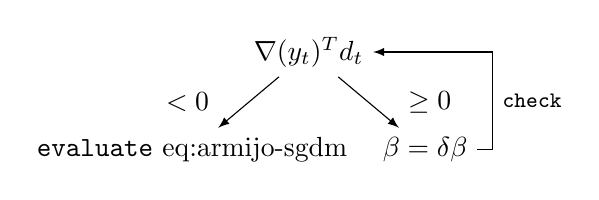
\begin{tikzpicture}
\node (A) at (0,0) {$\nabla\func(y_t)^Td_t$};
\node (B) at (-140:5.5em) {\texttt{evaluate}~\eqref{eq:armijo-sgdm}};
\node (C) at (-40:5.5em) {$\beta=\delta\beta$};
\draw[-latex] (A) -- node[left=2.5ex] {$<0$} (B);
\draw[-latex] (A) -- node[right=2.5ex] {$\geq0$} (C);
%\draw[-latex, bend right=55] (C.east) to (A.east);
\draw[-latex] (C.east) -- ++(0.2,0) -- node[right, font=\footnotesize] {\texttt{check}} ++(0,{5.5em*sin(40)}) -- (A.east);
\end{tikzpicture}
\end{center}
in algorithmic terms, until the direction is descent, damp the momentum term by a factor $\delta$, which is usually set to \num{0.5} like in the line search. Using this procedure, a descent direction $d_t$ is guaranteed and it is possible to apply the algorithm~\ref{alg:armijo}, the procedure is called \emph{momentum correction}, see algorithm~\vref{alg:m-correction}. The resulting algorithm is \texttt{MSL-SGDM-C}.

This procedure can be expensive, so the paper suggests another approach called \emph{momentum restart}, when the descent direction condition for $d_t$ isn't satisfied, the procedure restarts that direction by setting $d_{t-1}=d_0$, the paper suggests $d_0=0$, in general
\begin{center}
\begin{tikzpicture}
\node (A) at (0,0) {$\nabla\func(y_t)^Td_t$};
\node (B) at (-140:5.5em) {\texttt{evaluate}~\eqref{eq:armijo-sgdm}};
\node (C) at (-40:5.5em) {$d_{t-1}=d_0$};
\node (D) at ($(C) + (0,-1.5)$) {\texttt{evaluate}~\eqref{eq:armijo-sgdm}};
\draw[-latex] (A) -- node[left=2.5ex] {$<0$} (B);
\draw[-latex] (A) -- node[right=2.5ex] {$\geq0$} (C);
\draw[-latex] (C) -- node[right=1ex] {$d_t=-\bigl((1-\beta_0)\nabla f_{i_t}(y_t)+\beta_0d_0\bigr)$} (D);
\end{tikzpicture}
\end{center}
so if $d_0=0$ the direction will be $d_t=-(1-\beta_0)\nabla f_{i_t}(y_t)$ that is a descent direction, see algorithm~\vref{alg:m-restart}. The resulting algorithm is \texttt{MSL-SGDM-R}.

The authors suggest to set the momentum term to $\beta_0=0.9$.
